\documentclass[10pt,twocolumn,hidelinks]{IEEEtran}

\usepackage[boxed,commentsnumbered]{algorithm2e}
\usepackage{graphicx}
\usepackage{xcolor}
\usepackage{soul}
\usepackage{supertabular}
\usepackage{tabularx}
\usepackage{ caption, floatrow, makecell, booktabs}%
\usepackage{hyperref}
\setcounter{tocdepth}{1}
\usepackage{pdfpages}

\newcommand{\hlc}[2][yellow]{{%
    \colorlet{foo}{#1}%
    \sethlcolor{foo}\hl{#2}}%
}


\title{Analysing Algorithmic Patterns Based on Real Coding Interview Questions}
\author{\IEEEauthorblockN{Ian Dempsey,\\
Computer Science Department,\\
Maynooth University,\\
Email: ian.dempsey.2013@mumail.ie}
}
%\hlc[cyan!50]{_____} -> put in the stuff to be highlighted inside the {}
%cite{___} ->put in the bibtex key for the specific source.
%\label{sec: | fig: | } -> use to give something a specific label. This allows it to be referenced later
%\ref{___} -> to refernce a previously labeled area
\begin{document}
\tableofcontents
\addtocontents{toc}{~\hfill\textbf{Page}\par}
\listoffigures
\listoftables
\newpage
\maketitle
\pagenumbering{gobble}
\newpage
\pagenumbering{arabic}
\begin{abstract}
This paper aims to analyse and produce a report based off real world interview questions. This is being performed because programming questions have become staples in any interview with technology companies. To perform this analysis, this paper will simulate the interview environment by implementing restrictive time allowances for questions. This will allow the solutions created to be as authentic as possible. Every answer will be completed manually by the author of this paper, this allows for the human aspect of the interview process to be considered. To support the decision on which algorithm each solution is related to, control flow graphs have been designed for each standard algorithm to compare each solution to. By comparing the number of nodes and edges in the standard algorithm to the number of nodes and edges in the solution, it is possible to obtain a numerical value for the similarity between pieces of code. This numerical value is used to reinforce the decision on which algorithm a solution is close to. Overall this paper presents that learning the fundamental algorithms and patterns will allow a programmer of any experience to be a better programmer. By learning these algorithms, readers will able to spend more time thinking of the specific solution to a problem, once they identify which algorithm the question is most similar to. 
\end{abstract}
\section{Introduction}
\label{sec:intro}
\par
Nowadays interviews for jobs in the I.T industry are becoming more complex and demanding on the applicant. As this section of the working industry is usually quite technical, it is quite common for the applicants to have to perform some form of technical test. These tests normally involve several questions that are based on a wide variety of topics in programming. These questions are used to test potential employees on whether they have strong analytical and critical assessment skills. The technical tests also allow the employer to see how many standard algorithms the candidate knows, and can use. However, it is difficult to master all the different types of algorithms and their intricacies. 
\par The purpose of this paper is to study the relationship between the classical and well known algorithms, and the interview questions which are commonly asked.  This paper aims to give guidance to people who want to study the interview questions, but also learn a core set of common ideas which will help them solve multiple problems. This would therefore allow them to save time as they prepare for the interview.
\par This paper presents a comprehensive report summarising the similarities between interview questions and standard algorithms taught in a standard programming course. This distinguishes our work from interview preparation books which focus on the problem-solving skills, simply showing the reader a solution to a single problem, and not reinforcing material they would already be familiar with. 
\par The contribution of this paper can be summarised as the following: 
\begin{itemize}
\item Mastering the fundamental algorithms can cover a wide range of real world interview questions. 
\item We identify patterns that are closely related to these standard algorithms. 
\item We believe this paper can be used as a guidance for fresh graduates which can prepare them for real world interview questions.  
\end{itemize}
  %The questions themselves have a wide range of difficulty, from easier ones which focus on in basics of programming- e.g., array indexing, sorting algorithms, up to harder questions which really push candidates- e.g., dynamic programming, graphs. This area of interviewing is known as \textit{whiteboarding}, and has become quite common, it has led to some books being published which compile together numerous questions which are popular for interviewers to ask\cite{mcdowell2015cracking}.The focus in this paper is not the ability to solve as many quetions as possible to give to the applicants to study, but to try and discover patterns in problems which are similar, and then classify these patterns based off of pre-established patterns that candidates would be used to. This classification will then be able to help applicants and fellow programmers to learn how to see the patterns in problems quicker and be able to apply them to multiple problems, where they need only alter specific areas of code to solve the target problem. %
\section{Background}
\par Nowadays, in general, there are a lot of online repositories for interview questions and interview related material. Websites such as hackerrank.com, glassdoor.ie, geeksforgeeks.org, and leetcode.com all offer information on what questions are common during interviews for different companies. They also offer ways to test potential solutions to some of the given questions. 
\par For this paper we chose to use leetcode.com\cite{leet1}, as this website comes with a huge amount of online material that is generally taken from previously asked interview questions. Companies also use sites similar to leetcode when they are building up a bank of questions to pose to candidates. This was important in our decision for the repository, as it meant we were using a platform which was regularly updated. LeetCode itself also has some built-in features which greatly appealed to us. The website has an online discussion forum for each question, allowing the community to discuss solutions, issues, and the questions themselves. LeetCode also host their own weekly coding competitions which allow users to gain more experience and confidence in coding problems. One of the unique main features this online judge website has in comparison to others is a section for a user to perform a mock interview. This mock interview is under the time constraint of a normal real-world interview, this was a pre-eminent for us in choosing our online judge. The online editor that is used by leetcode also allows a user to select from a multitude of programming languages, as shown in Figure \ref{fig:langUI} below.
\par We chose Java for this project. The reason for this is because Java is widely used. However, our approach is applicable in other programming languages.  
\par The user interface of LeetCode is basic and accessible to use. The main page which lists all the problems, offers its users the option to filter questions by difficulty, which company has asked it before, what area the questions focuses on and much more. As seen in Figure \ref{fig:homepage}, we have chosen to focus on questions which are tagged as being related to trees. 
\begin{figure}[h]
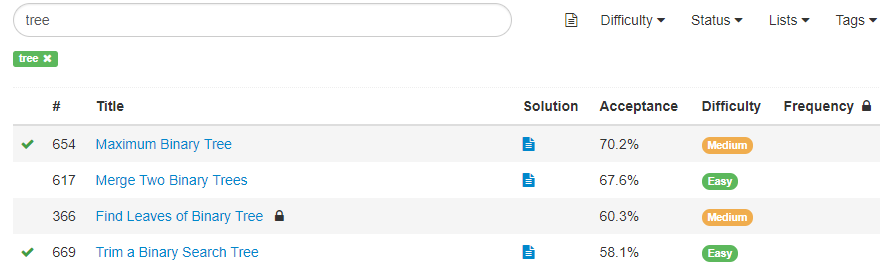
\includegraphics[scale=0.4]{homepageUI.png}
\caption{Homepage}
\label{fig:homepage}
\end{figure}

A user simply chooses the question which they wish to attempt, and is promptly brought to the problem's specific screen, as seen in Figure \ref{fig:problemPage}. On this screen there is a general description of the problem and a few examples for more clarification. This page also contains the online editor that the user will operate to attempt the problem. The online editor is intuitive to understand, and as stated has a variety of options for the user to choose from. 
\begin{figure}[h]
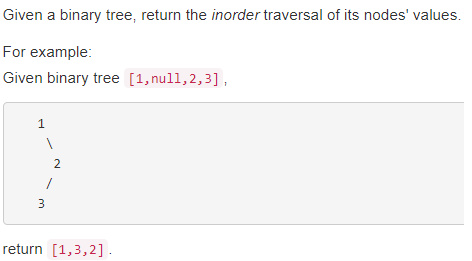
\includegraphics[scale=0.4]{problemPage.png}
\caption{Problem Specific Page}
\label{fig:problemPage}
\end{figure}

\begin{figure}[h]
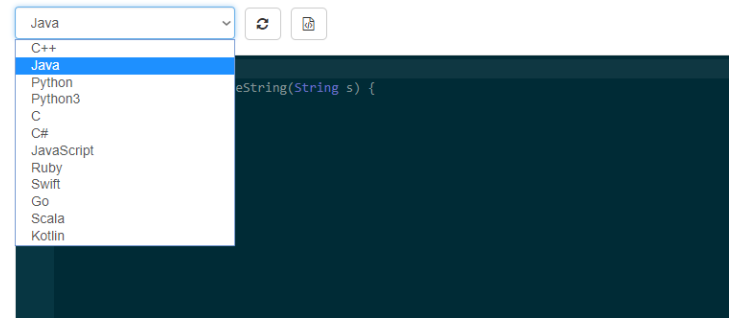
\includegraphics[scale=0.4]{languageUI.png}
\caption{Online editor with options displayed}
\label{fig:langUI}
\end{figure}   
The user will attempt to solve the problem they have selected, and they will then want to submit their answer and see if it is correct. They perform this by clicking the submit solution button underneath the editor. Leetcode allows a user to submit their code and be informed almost instantly if they are correct or not. There are two possible outcomes once the user clicks the submit button. Either it is accepted and leetcode returns an accepted result with suggestions for the next question a user could attempt, shown in Figure \ref{fig:accepted}, or their answer failed a certain testcase or even their code failed to compile and run, shown in Figure \ref{fig:fail}. In the case of failure, leetcode will report where an error is in the code by referencing the line.  
\begin{figure}[h]
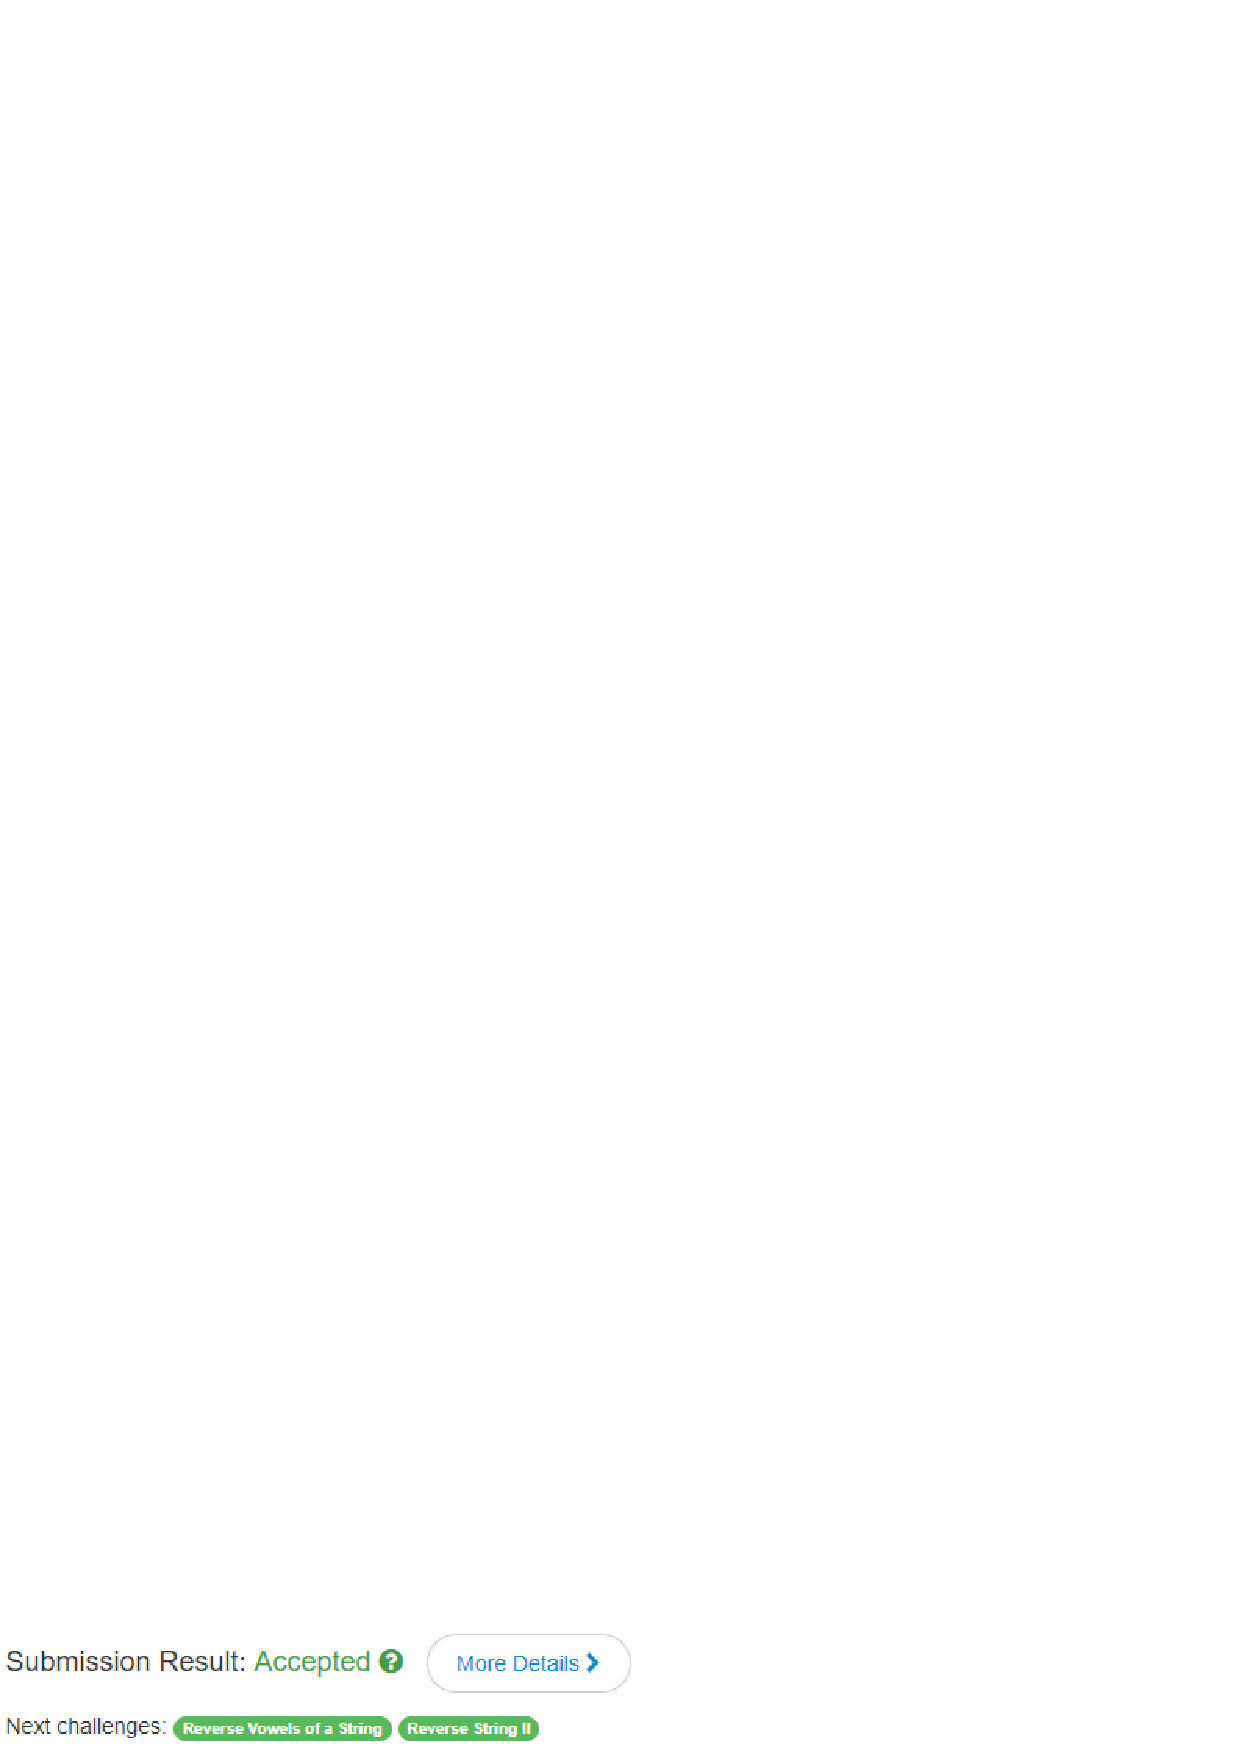
\includegraphics[scale=0.4]{accepted.png}
\caption{User solution passes all testcases}
\label{fig:accepted}
\end{figure}  
\begin{figure}[h]
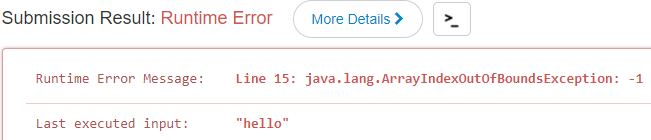
\includegraphics[scale=0.4]{failure.png}
\caption{User solution failing submission}
\label{fig:fail}
\end{figure}    

\section{Problem Statement}
\label{label:problemstmt}
We formulate the problem statement of this paper into the following three research questions:
\begin{itemize}
\item \textbf{RQ1: }What algorithms to choose, and what categories are these algorithms associated with. 
\item \textbf{RQ2: }How do these algorithms relate to the classic algorithms and how similar are they.
\item \textbf{RQ3: }How easy is it for a person to indentify the pattern of the algorithm.
\end{itemize}

\section{The Solution}
To answer RQ1, we first collect some useful information. For example many companies took their questions from online repositiories such as Glassdoor \cite{glassdoor}, and websites which discussed experiences people had at interviews. We also read through some interviewing preparing books. These books typically list a range of topics covered in interviews, such as Cracking the Coding Interview covers Binary Search, Dynamic Programming and Graph Traversal \cite{mcdowell2015cracking}. Further many websites publish the top real world interview questions. This is based on the user interview experience. For example geeksforgeeks has a list of the top interview questions that a user should study prior to an interview, for example Linked Lists, Binary Search Trees and Sorting \cite{geeksalgos}. For these reasons, this paper focuses on the following algorithms:

\begin{table}[h]
\centering
	\begin{tabular}{| c | } \hline
		   Algorithms \\ \hline
		Sorting Algorithms\\ \hline
		Searching Algorithms\\ \hline
		Graphs  \\ \hline
		Trees  \\ \hline
		Dynamic Programming \\ \hline
	\end{tabular}
	\caption{Algorithms chosen for this project}
	\label{tab:fiveareas}
\end{table}
In each of these areas we categorise them into seven key patterns (see Table \ref{tab:classicalAlgos}). These are patterns or types of the above listed algorithms which commonly appeared.
 
\par Among the many websites and interview books, we discovered Leetcode is possibly the bets resource for preparing for interviews. Therefore we select around fourty questions. Those fourty questions are representative of the five areas that this paper forcuses on \ref{tab:fiveareas}.They were selected based on reputation, if they were asked in interviews, and the pass rate of the question. Relating back to Figure \ref{fig:homepage}, it can be seen that questions can be filtered. Leetcode has over six hundred questions, which is impossible to answer in such a short period of time.
\par With regards to RQ2, in order to find the most similar algorithm, we first compared the ideas of the classical algorithm and the solution to the question we were solving. It is possible to have multiple algorithms apply to a problem. We implemented the easiest solution which is the first which came to our minds. This is because one normally has limited time in an interview, and this means that a person would build on an idea they initially discover after they understand the question being asked. The candidate would not have enough time to explore multiple solutions to a problem under the interview conditions. 
\par To try and obtain a numerical representation of similarity between the standard algorithm and the solution we created, we decided to count how many edit operations we require to transform one piece of code into another and these edits are categorised into two operations, adding and deleting code.
As this would be a considerable task to perform by hand, we used an online difference calculator called DiffChecker \cite{diff} to get the differences between the two source files, A and B. DiffChecker returns the number of edit operations, additions and deletions, required to transform one piece of code into the other. Then we went through the listed changes manually, we did this to verify the changes that DiffChecker suggested to us were required to make the two pieces of code identical in logical terms.This process was not automatic and therefore needed to be improved. 
\par We also looked into using tools for plagiarism checking such as Turnitin and Moss \cite{Schleimer:2003:WLA:872757.872770}. Moss is a powerful tool for detecting plagiarism. Moss is described as an automatic system for determining the similarity of programs \cite{mosswebsite}. The tool itself is heavily focused on finding plagiarised pieces of code from given sources. Even though there were benefits of using Moss, as documented by other users \cite{MossBowyer}, we decided not to use it. This was for a few reasons, mainly that the process was quite laborious, as we needed to send off each file to compare with a base file. 
\par Finally it was decided that the use of control flow graphs would be beneficial to obtaining a numerical value for the similarity between pieces of code. The use of control flow graphs is explained later on in the section \ref{label:CFG}.
\par We have listed the aforementioned patterns in the following section, along with sample questions which are similar to the classical algorithms. We picked only a few to represent all of the questions due to the page limit. Please see Table \ref{tab:tabSols} for more detail.
\subsection{Palindrome}
Palindromes are extremely useful for searching. As Palindromes are meant to be the same in both directions, one can easily discover if the input is an actual palindrome. This is helpful for searching because one can search and find the odd character out, or the unique piece of data in some text. This style of algorithm is also space efficient, they normally have a space analysis of O(n/2) as the algorithm works over two elements of the input at a time. The basic approach of a Palindrome algorithm is to work inwards with both pointers starting at either end of the input and constantly moving towards one another and comparing if the elements are the same.\\  
Algorithm \ref{fig:pal} is a general algorithm for solving the palindrome problem which is a common problem in java and other languages. This approach can be used to solve numerous other problems by altering the inside of the loop.
\IncMargin{1em}
\begin{algorithm}
	\LinesNumbered
	\SetKwInOut{Input}{Input}
	\SetKwInOut{Output}{Output}
	\Input{Given input of characters, S}
	\Output{Boolean}
	$leftIndex  \longleftarrow $S[0]\\
	$rightIndex \longleftarrow $S.length-1\\
	\While{leftIndex $<$ rightIndex}{	
		compare leftIndex with rightIndex \\
		\If{leftIndex !=rightIndex}{
			return false \\
		}
	 	leftIndex++ \\
		rightIndex++\\
	}
\Return true
\caption{The Palindrome Algorithm}
\label{fig:pal}
\end{algorithm}\DecMargin{1em}
 \textbf{ID 1} TwoSum is one example where the Palindrome algorithm was used to solve the question. This question is described as: \textit{''Given an array of integers, return indices of the two numbers such that they add up to a specific target. You may assume that each input would have exactly one solution, and you may not use the same element twice.''} Algorithm \ref{fig:twosum} is the solution accepted by LeetCode. In this pseudocode we have highlighted any differences in blue, this is the same for all the following answers.
\IncMargin{1em}
\begin{algorithm}
	\LinesNumbered
	\SetKwInOut{Input}{Input}
	\SetKwInOut{Output}{Output}
	\Input{Array of integers nums, target S}
	\Output{Indices i,j}
	$leftIndex  \longleftarrow $S[0]\;
	$rightIndex \longleftarrow $S.length-1\;
	\While{leftIndex $<$ rightIndex}{
	\hlc[cyan!50]{Sort the input array nums\;}\\
	\uIf{\hlc[cyan!50]{nums[leftIndex]+nums[rightIndex] $>$ S}}{
		\hlc[cyan!50]{rightIndex$--$\;}
	}\uElseIf{\hlc[cyan!50]{nums[leftIndex]+nums[rightIndex]$<$S}}{
		\hlc[cyan!50]{leftIndex++\;}
	}\Else{
		\Return\hlc[cyan!50]{ leftIndex, rightIndex\;}
	}
     }\Return 0\;
\caption{LeetCode Q1 TwoSum}
\label{fig:twosum}
\end{algorithm}\DecMargin{1em}\\
As can be seen in Figure \ref{fig:twosum}, the main differences are the conditionals inside the while loop. The conditionals will only move one pointer at a time, depending on the result of adding the two current elements at each pointer together. If the total is greater than the target sum, then the right-pointer is moved left once, as this would allowthe sum to be smaller and potentially the correct sum. If on the other hand the sum was smaller than the total, then the left-pointer is moved right once, the two elements are added together resulting in a new total. This process was repeated until the target sum was found, or until the two pointers crossed which meant the target was not found.

\subsection{Merge Sort}
Merge Sort is a very powerful algorithm. It is more efficient than most styles of insertion, with a time analysis of $O(n * log_{n})$, whereas insertion is $O(n^2)$. The idea of merge sort is to divide an array or some input in half and then sort each half before joining it back together. They do not have to be the same size which is useful.  \\
Merge Sort uses the idea of divide and conquer, this means the list to be sorted should be divided up into equal parts first, then these new smaller parts should be sorted individually before recreating the full list. Algorithms \ref{fig:mergesort} and \ref{fig:merge} show this.
\IncMargin{1em}
\begin{algorithm}
	\LinesNumbered
	\SetKwInOut{Input}{Input}
	\SetKwInOut{Output}{Output}
	\Input{List of unsorted data A, int left, int right}
	\Output{Sorted List}
 	\eIf{ left == right}{ \Return A[left]}
  	{$mid \longleftarrow (left+right)/2$\;
  	$recMergeSort(A,left,mid)$\;
  	$recMergeSort(A,mid+1,right)$\;
  	$merge(A,left,mid+1,right)$
  	}
\caption{recMergeSort(). The Merge Sort Algorithm through Recursion}
\label{fig:mergesort}
\end{algorithm}\DecMargin{1em}

\IncMargin{1em}
\begin{algorithm}
	\LinesNumbered
	\SetKwInOut{Input}{Input}
	\SetKwInOut{Output}{Output}
	\Input{List of unsorted data A, int left, int mid, int right}
	\Output{Sorted List A}
 	$n1 \longleftarrow mid - left + 1$ ; $n2 \longleftarrow right - mid$\;
 	$temp1[] \longleftarrow [n1]$  ; $temp2[]\longleftarrow [n2]$\;
 	\tcc*[h]{Copy data into each temparray}
 	\For{$i\leftarrow 1$ \KwTo $n1$}{copy}
	\For{$i\leftarrow 1$ \KwTo $n2$}{copy}
	$i \longleftarrow $0 ; $j \longleftarrow $0 ; $k \longleftarrow $left
	\While{$i < n1$ \&\& $j < n2$}{
	\If{$temp1[i] <= temp2[j]$ }{
		$A[k] = temp1[i]$; $i++$
	}
	\Else{
		$A[k] = temp2[j]$; $j++$
		}
		$k++$
	}
	\While{$i < n1$}{
		$A[k] = temp1[i]$; $i++$; $k++$
	}
	\While{$j < n2$}{
		$A[k] = temp2[j]$; $j++$; $k++$
	}
	\Return A
\caption{merge(). The merge method for Merge Sort}
\label{fig:merge}
\end{algorithm}\DecMargin{1em}

\par As can be seen, the Merge Sort is quite a long algorithm, which contains many intricate parts which must be correct inorder for the algorithm to work correctly. \textbf{ID 23} \textit{Merge K Sorted Lists} is an example of Merge Sort being used to solve a problem. 
The question is defined as: \textit{'' Merge k sorted linked lists and return it as one sorted list. Analyze and describe its complexity.''} Algorithms \ref{fig:mergeK} and \ref{fig:mergeK2} is the solution to this question.
\IncMargin{1em}
\begin{algorithm}
	\LinesNumbered
	\SetKwInOut{Input}{Input}
	\SetKwInOut{Output}{Output}
	\Input{ListNode[]A, int left, int right}
	\Output{Sorted List[] A}
 	\eIf{ left == right}{ return A[left]\;}
  	{$mid \longleftarrow $(left+right)/2\\
  	 \hlc[cyan!50]{$l1 \leftarrow recMergeSort(A,left,mid)$\\}
  	\hlc[cyan!50]{$l2 \leftarrow recMergeSort(A,mid+1,right)$\\}
  	\hlc[cyan!50]{$merge(l1,l2)$}\tcc*[h]{See Algorithm \ref{fig:mergeK2}}\; 
  	}
\caption{recMergeSort() function Merge K Sorted Lists}
\label{fig:mergeK}
\end{algorithm}\DecMargin{1em}

\IncMargin{1em}
\begin{algorithm}
	\LinesNumbered
	\SetKwInOut{Input}{Input}
	\SetKwInOut{Output}{Output}
	\Input{ListNode l1, ListNode l2}
	\Output{Sorted List}
	\If{\hlc[cyan!50]{l1 == null}}{
		\hlc[cyan!50]{return l2}
	}
	\If{\hlc[cyan!50]{l2 == null}}{
		\hlc[cyan!50]{return l1}
	}
	\If{\hlc[cyan!50]{$l1.val < l2.val$}}{
		\hlc[cyan!50]{l1.next = merge(l1.next,l2)}\\
		\hlc[cyan!50]{return l1}
	}
	\hlc[cyan!50]{l2.next = merge(l1,l2.next)}\\
	\hlc[cyan!50]{return l2}
\caption{merge() function for \textbf{ID 23}}
\label{fig:mergeK2}
\end{algorithm}\DecMargin{1em}
\par Comparing this solution which is based off of Merge Sort, it can be seen that the main difference is inside the merge method, Algorithm \ref{fig:mergeK2}. The reason for this is because each scenario will alter the merge method due to their data structures and requirements. On the other hand, Algorithm \ref{fig:mergeK} is very similar to the standard pattern.  
\subsection{Binary Search}
Binary Search is a rapid algorithm for locating data. It has a time complexity of $O(log{n})$ and is used when working with sorted arrays. The algorithm is also used when using binary search trees. In this section the examples are shown with arrays. This algorithm compares the target value to the middle value of the array. If the target is less than this middle value, then the upper half is eliminated as the target cannot lie in this section and the search continues on the remaining half until the search is successful or not. Algorithm \ref{fig:binary} shows the standard binary search algorithm.
\IncMargin{1em}
\begin{algorithm}
\LinesNumbered
	
	\SetKwInOut{Input}{Input}
	\SetKwInOut{Output}{Output}
	\Input{Sorted array S, target x}
	\Output{index of target or -1}
	$left \longleftarrow $0 ; $right \longleftarrow $S.length-1\\
	\While{left $<=$ right}{
		$mid \longleftarrow $left + (right - left)/2\\
		\If{S[mid] $==$ x}{
			\Return $mid$
		}
		\If{S[mid]$<$x}{
		$left = mid + 1$
		}
		\Else{
		$right = mid-1$
		}
	}
	\Return -1
\caption{Binary Search}
\label{fig:binary}
\end{algorithm}\DecMargin{1em}

\textbf{ID 69} \textit{Sqrt(x)}, is just one example of binary search being employed to solve a question. This question is described as: \textit{''Implement int sqrt(int x). Compute and return the square root of x. x is guaranteed to be a non-negative integer.} Algorithm \ref{fig:sqrt} is the solution to this problem. 
\IncMargin{1em}
\begin{algorithm}
\LinesNumbered
	
	\SetKwInOut{Input}{Input}
	\SetKwInOut{Output}{Output}
	\Input{Int x}
	\Output{Int y}
	\If{\hlc[cyan!50]{x $==$ 0}}{ \Return \hlc[cyan!50]{0}}
	$left \longleftarrow 1$ ; $right \longleftarrow x/2$\\
	\While{true}{
		$mid \longleftarrow $left + (right - left)/2\\
		\If{\hlc[cyan!50]{mid $>$ x/mid}}{
			$right = mid-1$
		}
		\Else{
		\If{\hlc[cyan!50]{$mid+1 > x/(mid+1)$}}{
			\Return \hlc[cyan!50]{$mid$}
			}
			\hlc[cyan!50]{$left = mid+1$}
		}
	}
\caption{Sqrt(x)}
\label{fig:sqrt}
\end{algorithm}\DecMargin{1em}
\par A second example of a question from leetcode.com which is based off of binary search is \textbf{ID 441} Arranging Coins. The description for this questions is given as: \textit{''You have a total of n coins that you want to form in a staircase shape, where every k-th row must have exactly k coins. Given n, find the total number of full staircase rows that can be formed. n is a non-negative integer and fits within the range of a 32-bit signed integer.''} Algorithm \ref{fig:arrangingcoins} is the solution to this problem.  
\IncMargin{1em}
\begin{algorithm}
	\LinesNumbered
	\SetKwInOut{Input}{Input}
	\SetKwInOut{Output}{Output}
	\Input{Int n}
	\Output{Number of full steps completed}
	$low\longleftarrow $1\;
	$high \longleftarrow $\hlc[cyan!50]{n}\;
	\While{low $<=$ high}{
		$mid \longleftarrow $low + (high - low)/2\;
		\If{\hlc[cyan!50]{mid $*$ (mid+1L) $<=$2L$*$n }}{
			low $=$ mid+1\;
		}
		\Else{
			high = mid -1\;
	}
}\Return \hlc[cyan!50]{high}\;
\caption{Arranging Coins}
\label{fig:arrangingcoins}
\end{algorithm}\DecMargin{1em}
\par As is detailed in Algorithm \ref{fig:arrangingcoins}, this solution is extremely close to the original pattern for binary search. The first change of note is within the assignments at the start. This is where the variable \textit{high} is set to n. This is so the calculation starts at n, as this is the upper limit and max number of steps that could theoretically be produced. The main change required is in the first conditional, which when returns true means that the lower side must be moved up, so \textit{low} is reset to be mid + 1.
	
	\subsection{Graphs}
	Graphs are common in our lives. News media use them to help us visualize certain statistics. Though these are not the graphs that are studied by Computer Scientists. Graphs studied by Computer Scientists are usually based on the tree structure, and the relationships 	among data elements. A tree is just one of the special types of graphs that can be studied, where the parent-child relationship is used to organise data. In this section I have focused on the Tree Abstract Data Type, Breadth-First Traversal, Depth-First Traversal and Graphs in general. \\
	\subsubsection{Trees}
	Trees are one of the most powerful styles of data structures for processing data, this is because they allow rapid searching and fast insertion/deletion of a node. Trees are made up of nodes, which are objects which hold some data and have a key. This key allows one to determine where this node should be in the tree. The important distinction here with these nodes in comparison to other nodes used in various data structures, is that these nodes contain references to children instead of just the next Link. Each node has exactly one parent, but can have many children. A Binary Search Tree is a special type of tree, this is a tree which has strictly between zero and two children and keeps their keys in sorted order. It has $O(n)$ space, search, insertion and deletion operations. 
	\par With trees the main function is traversal. There are three basic styles of traversal: inorder, preorder and postorder. Inorder visits every node in the left subtree, the root and then the right subtree. Preorder is where the root is visited first, followed by its left subtree and then it's right subtree. Finally, postorder is where the left subtree is followed by the right subtree and then the root. \\
Algorithm \ref{fig:nodesearch} is an example of how one might search for a particular node in a Tree.\\
\IncMargin{1em}
\begin{algorithm}
	\LinesNumbered
	\SetKwInOut{Input}{Input}
	\SetKwInOut{Output}{Output}
	\Input{Given a key to search for}
	\Output{The desired Node, or null}
	$Node current \longleftarrow root$\;
	\While{current.data is not key}{
		\If{current is null}{\Return $null$}
		\eIf{current.data $>$ key}{
			move left on the tree\\
		}{
		move right on the tree\\
		}
	}
\Return $current$\;
\caption{Finding a specific Node in a tree based on the key}
\label{fig:nodesearch}
\end{algorithm}\DecMargin{1em}
\\
\IncMargin{1em}
\begin{algorithm}
\SetAlgoNoLine
\LinesNumbered
	\SetKwFunction{postOrder}{postOrder}
	\Indm\postOrder{$Node$ $localRoot$}
	\\
		\If{localRoot $!=$ null}{
		$\postOrder(localRoot leftChild)$\\
		$\postOrder(localRoot rightChild)$\\
		$Print(localRoot data)$\;}	
\caption{Basic Tree Traversal using PostOrder Traversal}
\label{fig:postorder}
\end{algorithm}\DecMargin{1em}
\par Algorithm \ref{fig:postorder} is the basic postorder traversal of a tree. The key area to note is thr order of calling the different children of a node. Altering this will result in preorder and inorder traversal.

\par \textbf{ID 104}, \textit{Maximum Depth of Binary Tree}, is an example of a problem where the basic tree traversal styles were used to solve the question. The problem description is given as: \textit{''Given a binary tree, find its maximum depth. The maximum depth is the number of nodes along the longest path from the root node down to the farthest leaf node.''} Postorder traversal was used. Pseudocode can be found in Figure \ref{fig:maxdepth} of this paper.\\
\IncMargin{1em}
\begin{algorithm}
\SetAlgoNoLine
\LinesNumbered
	\SetKwFunction{maxDepth}{maxDepth}
	\Indm\maxDepth{$TreeNode$ $localRoot$}\\
		\If{\hlc[cyan!50]{localRoot $==$ null}}{\Return \hlc[cyan!50]{0\;}}
		\Else{
		\hlc[cyan!50]{int ldepth $=$}\maxDepth(localRoot leftChild)\\
		\hlc[cyan!50]{int rdepth $=$}\maxDepth(localRoot rightChild)\\
		\If{\hlc[cyan!50]{ldepth $>$ rdepth}}{
		\Return  \hlc[cyan!50]{ldepth+1\;}
		}\Else{ \Return \hlc[cyan!50]{ rdepth+1\;}}
		}
\caption{Leetcode Q104 Max. Depth of Binary Tree}
\label{fig:maxdepth}
\end{algorithm}\DecMargin{1em}
\\
As highlighted in Algorithm \ref{fig:maxdepth}, the key difference is inside the if statement. The conditional is the base case to stop the recursive execution on the stack. Variable \textit{ldepth} is the total depth of the left subtree. This is a recursive call on the leftChild of the current node. Line 4 will execute until it can't go left anymore, if it reaches null it will try to go right once, and then return going left. This is repeated until both calls return null. The stack then returns all the recursive calls on it, adding them together and seeting them to \textit{ldepth}. This process is repeated on the right subtree, and set it to the variable \textit{rdepth}. Finally, there is a conditional checking if ldepth is greater than rdepth. If so it returns ldepth+1, or it returns rdepth+1. This +1 is required as we need to consider the root node's level, if we didn't take this into account the answer would always be one less than the actual depth of the tree. The major similarities between the postorder algorithm and this solution is the recursive call to traverse the left subtree first, then the right subtree and finally to take the root into account by adding 1. This way of traversing the tree, left-right-root, is exactly how postorder traversal is performed.
\\
\subsubsection{Breadth-First Search}
This is a special way to visit the nodes in a tree, the ordering in this traversal pattern is to visit the root node, then move onto the children of the root node, printing each child in turn. It then will repeat this for each child of these nodes. Figure \ref{fig:breadth} shows the nodes in numerical order of visitation when using Breadth-First Search. \\
\begin{figure}[h]
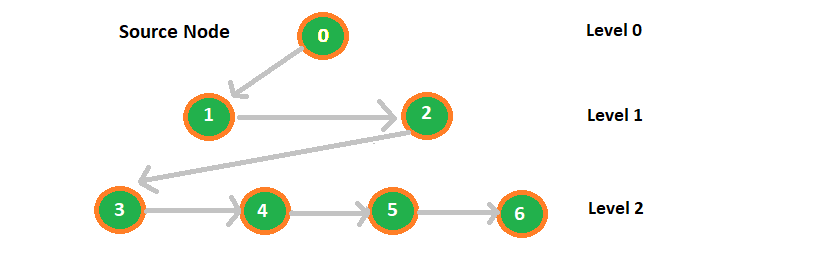
\includegraphics[scale=0.5]{bfs.png}
\caption{Breadth-First Search}
\label{fig:breadth}
\end{figure}
 \\
\subsubsection{Depth-First Search}
This is a second way of visiting nodes in a tree. This pattern involves starting at the root node, then going to the left most child, then repeating this movement until the traversal reaches a leaf node (a node which has no children), then it will move back up one node and try to visit the next child node of this current node. It repeats this until the traversal finds no unvisited node. Figure \ref{fig:depth} shows the nodes in numerical order of visitation when using Depth-First Search. 
\begin{figure}[h]
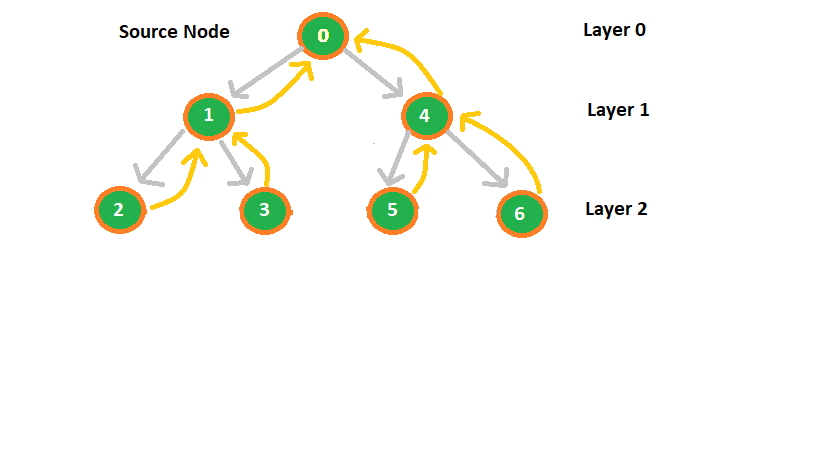
\includegraphics[scale=0.5]{dfs.png}
\caption{Depth-First Search}
\label{fig:depth}
\end{figure}

\subsection{Dynamic Programming}
Dynamic Programming is outlined as `smart recursion'. This is because it takes the idea of recursion and improves on the inefficiencies of recursion. These inefficiencies mainly being that recursive algorithms are generally space inefficient. Each recursive call adds a new layer to the stack. Therefore, dynamic programming is such a strong style of programming as it uses the simplicity of recursion but does not have the problem of causing a stack overflow. Dynamic programming  is described as taking a recursive algorithm and finding the overlapping subproblems. A user then caches these results for future recursive calls.
This style is known as \textit{Top-Down}. There is a different approach, known as \textit{Bottom-Up}. We will give a quick demonstration of the two by using the classic recursive algorithm to solve Fibonacci numbers.
\IncMargin{1em}
	\begin{algorithm}
	\LinesNumbered
		%\Fn(\tcc*[h]{recursive fibonacci}){\FRecurs{Integer n}}{
		\SetKwInOut{Input}{Input}
		\SetKwInOut{Output}{Output}
		
		\Input{Integer n}
		\Output{Fibonacci Numbers}
		\If{n$<$3} {\Return 1\\}
		\Return $fib(n-2) + fib(n-1)$
			
	\caption{Fibonacci Numbers through normal recursion}
	\end{algorithm}
\DecMargin{1em}
	
	\subsubsection{Top-Down}
	This method of dynamic programming follows the normal structure of a simple recursive solution. Start from n and compute smaller results as they are needed to solve the original problem. Results are stored in some form of data structure, this is known as memoization. These stored results can be accessed quickly and efficiently in comparison to having to recompute the same values for n repeatedly. This leads to saving space on the stack, and time when working with recursively styled problems. See Algorithms \ref{fig:topdown1} and \ref{fig:topdown}.
	
\IncMargin{1em}
	\begin{algorithm}
	\LinesNumbered
		\SetKwInOut{Input}{Input}
		\SetKwInOut{Output}{Output}
		\Input{Integer n}
		\Output{Fibonacci Numbers}
		$computed \leftarrow $HashMap\;
		\If{n$<$3} {\Return 1\\}
		\Return $fib(n-2) + fib(n-1)$\\
		$computed put (1,1)$\\
		$computed put (2,1)$\\
		\Return $fib2(n, computed)$\\
		\caption{fib; Fibonacci Numbers through Top-Down and Memoization}
		\label{fig:topdown1}
	\end{algorithm}\DecMargin{1em}
\IncMargin{1em}
	\begin{algorithm}
	\LinesNumbered
		\SetKwInOut{Input}{Input}
		\SetKwInOut{Output}{Output}
		\Input{Integer n, HashMap computed}
		\Output{Fibonacci Number}
		\If{computed containsKey(n)} {\Return $computed get(n)$\\}
		$computed.put(n-1,fib2(n-1,computed))$\\
		$computed.put(n-2,fib2(n-2,computed))$\\
		$newVal \leftarrow computed.get(n-1) + computed.get(n-2)$\\
		\Return $newVal$\\
	\caption{fib2;Fibonacci Numbers through Top-Down and Memoization}	
	\label{fig:topdown}
	\end{algorithm}\DecMargin{1em}	
	
	
	\subsubsection{Bottom-Up}
	The issue with the Top Down version is that even though the results are being saved to reuse later, they must be calculated from n to the base cases through recursion the first time. This is performed only once, when no values have been computed, so nothing has been stored.
	Bottom-Up solves this by going in reverse to the normal recursive way. Instead of starting at n and working down towards the base case, it works its way up to the value of n. See Algorithm \ref{fig:bottomup}.
\IncMargin{1em}
	\begin{algorithm}
	\LinesNumbered
		\SetKwInOut{Input}{Input}
		\SetKwInOut{Output}{Output}
		\Input{Integer n}
		\Output{Fibonacci Numbers}
		\SetKwArray{Kw}{results}
		$results[] \leftarrow int[n+1]$ ; $results[1] = 1$ \\ $results[2] = 2$ \\
		\For{$i \leftarrow 3$ \KwTo $n$}{ 
		$results[i] = results[i-1]+results[i-2]$\\}
		\Return $results[n]$\\		
		\caption{fibDP; Fibonacci Numbers through Bottom-Up}
		\label{fig:bottomup}
	\end{algorithm}\DecMargin{1em}
	\\
\par It must be noted though that Dynamic Programming is one of the toughest sections of programming to learn. This only makes it more challenging for candidates to answer questions in interviews in such a limited window. The reason it is so tough is because a candidate must think of the problem in multiple ways, and make the decision to tackle it in a certain manner. If they choose the wrong option, then they will end up with a very inefficient solution, choose correctly and they will have shown a very strong understanding of this area.
\section{Evaluation}
In the previous section of this paper, only specific examples of the solutions were shown. Here we give a detailed summary of all solved questions in Table \ref{tab:tabSols}. These were accepted by leetcode's online judging system. 
We also have created a table which details a numeric value for the algorithms previously listed in the solution section.
\begin{table}
\parbox{.45\linewidth}{
\centering
\begin{tabular}{|c|c|}
		    &Algorithms \\ \hline
		1 & Palindrome\\ \hline
		2 & Merge Sort\\ \hline
		3 & Binary Search\\ \hline
		4 & Tree Traversal \\ \hline
		5 & Breadth-First Search\\ \hline
		6 & Depth-First Search\\ \hline
		7 & Dynamic Programming\\ \hline
		- & None required\\ \hline
\end{tabular}
\caption{The classical algorithms and data structures}
\label{tab:classicalAlgos}
}
\hfill
\parbox{.45\linewidth}{
\centering
\begin{tabular}{|c|c|}
	&Data Structures \\ \hline
	1 & List\\ \hline
	2 & Trees\\ \hline
	3 & Stacks\\ \hline
	4 & Queues \\ \hline
	5 & Arrays\\ \hline
	6 & Maps\\ \hline	
	7&Strings\\ \hline
	-&None required\\
\end{tabular}
}
\end{table}

\begin{table}[t]
\begin{tabular}{|c| c| c| c| c| c|} \hline
 Question ID & PassRate & Difficulty & Time(mins) &Evaluation &Algorithm \\
	 \hline
 	1 & 36.0\% & Easy & 9 & Easy & [1,[5]]\\ 
 	\hline
	 2 & 28.1\% & Medium & 20 &Medium& [-.[1]]\\
 	\hline
	 20 & 33.7\% & Easy & 12&Easy& [1,[3]] \\
 	\hline
 	21 & 39.3\% & Easy & 25&Easy& [-,[1]] \\
 	\hline
 	23 & 27.7\% & Hard & 27&Medium&[2,[1,5]] \\
  	\hline
 	35 &39.8\%  & Easy & 10 &Easy&[-,[5]]\\
  	\hline
 	53 &39.9\%  & Easy & 20 &Medium& [-,[5]]\\
  	\hline
 	58 & 32.0\% & Easy & 15 &Easy&[-,[5,7]]\\
  	\hline
 	69 & 28.2\% & Easy & 19 &Easy&[3,[-]]\\
  	\hline
 	70 & 40.5\% & Easy & 18 &Easy&[7,[5]]\\
 	\hline
 	72 & 32.1\% & Hard & 29 &Hard&[7,[5]]\\
  	\hline
 	88 & 32.1\% & Easy & 12 &Medium&[-,[5]]\\
  	\hline
 	94 & 47.8\% & Medium & 27 & Medium&[4,[1,2,3]]\\
  	\hline
 	102 & 40.9\% & Medium & 30  &Medium & [5,[1]]\\
  	\hline
	104 & 53.5\% &Easy  &28  &Medium& [4,[2]]\\
  	\hline
 	111 &  33.3\%& Easy&17  &Easy& [5,[2,4]]\\
  	\hline
 	114 & 35.7\% &Medium  & 33  &Medium&[4,[2]]\\
  	\hline
 	136 &54.9\%  &Easy  &10  &Easy& [-,[5]]\\
  	\hline
 	147 & 33.4\% &Medium  &26  &Medium& [-,[1]]\\
	\hline
 	152 &  26.2\%& Medium & 31 &Hard&[7,[5]]\\
  	\hline
  	167 & 47.1\% &Easy  &16  &Easy&[1,[5]]\\
  	\hline
  	169 & 47.3\% &Easy  &20  &Easy&[-,[5]]\\
  	\hline
  	205 & 34.2\% &Easy  &18  &Easy& [-,[6]]\\
  	\hline
  	230 & 44.1\% &Medium  &19  &Medium&[4,[2,3]]\\
  	\hline
 	290 & 33.2\% &Easy  &28  &Medium&[-[5,6]]\\
  	\hline
 	326 & 40.4\% &Easy  &25  &Easy&[-[-]]\\
   	\hline
  	336 & 26.5\% &Hard &18  &Medium&[1,[1,7]]\\
  	\hline
 	344 & 59.5\% &Easy  &8  &Easy&[1,[5,7]]\\
  	\hline
 	387 & 47.1\% &Easy  & 19 &Medium&[-,[5]]\\
  	\hline
 	389 & 50.9\% &Easy  & 10 &Easy& [-,[5]]\\
  	\hline
 	404 & 47.3\% &Easy  &16  &Medium&[4,[2]]\\
	\hline
 	441 & 36.3\% &Easy  &6&Easy &[3,[-]]\\ 	
  	\hline
 	654 & 70.1\% &Medium  &46  &Hard&[2,[2,5]]\\
  	\hline
	669 &  58.1\%& Easy &18  &Easy&[4,[2]]\\
  	\hline
	687 &  33.5\%& Easy &21  &Medium&[-,[2]]\\
  	\hline
 	690 &  52.9\%& Easy &   45&Medium&[5,[3,6]]\\[1ex]
 	\hline
\end{tabular}
\caption{All solutions}
\label{tab:tabSols}
\end{table}
\par In Table \ref{tab:tabSols} there a number of headings. Question ID is the specific ID of each question solved. PassRate is the percentage of solutions accepted by leetcode. These were taken at the time of writing. Difficulty is the level that was awarded to each question by LeetCode. Time is the total time in minutes it took to complete each question. Evaluation is our opinion on the difficulty of each question. Algorithm, this is the algorithm and data structures which were used to solve the question. The first number in the list refers to the algorithm, the second list refers to the relevant data structures used. Both can be found in Table {\ref{tab:classicalAlgos}}

\par As can be seen in Table \ref{tab:tabSols}, some of the questions which were marked as having difficulty easy, took longer than some which were marked as medium. This is because it took longer for the pattern which was useful to solve the problem to be discovered.
\par It is not easy to judge how fast a user can detect the underlying pattern of a problem. This is because each user will have a different background. We have categorised the different users into four distinct types. 
\begin{enumerate}
\item{People which have a background in coding competitions. They are highly experienced and are unlikely to find the questions hard.}
\item{Users with some computer science background, who understand the internal workings of data structures and other concepts. These people would generally find most problems approachable.}
\item{People who understand basic concepts. They will struggle with the advanced topics.}
\item{People who are interested in learning to code who have no experience. They will have to put a lot of study in to grasp basic concepts.}
\end{enumerate}
This leads to the creation of Table \ref{tab:difficulty}, in whicheach type of user is paired with the expected difficulty they would face answering the questions on leetcode.com. 
\begin{table}[t]
\centering
	\begin{tabular}{| c | c |} \hline
		   Background Type &Expected Difficulty \\ \hline
		1 & Easy \\ \hline
		2 & Medium \\ \hline
		3 & Medium  \\ \hline
		4 & Hard  \\ \hline
	\end{tabular}
	\caption{The expected difficulty each type of categorised user would have with the questions.}
	\label{tab:difficulty}
\end{table}

\subsection{Question Evaluation}
Whilst working on the numerous questions that were solved,  some issues did arise which related to the questions themselves. These problems stemmed from the questions being worded strangely, or the example given for the solution was not explicitly clear in the way the question worked. These were just some of the issues which occurred whilst attempting to solve the problems. An example of such an issue is \textbf{ID} 654, Maximum Binary Tree. This question's problem was easy to understand:
\\ \textit {''Given an integer array with no duplicates. A maximum tree building on this array is defined as follow:
\begin{enumerate}
\item The root is the maximum number in the array.
\item The left subtree is the maximum tree constructed from left part subarray divided by the maximum number.
\item The right subtree is the maximum tree constructed from right part subarray divided by the maximum number.
\end{enumerate}
Construct the maximum tree by the given array and output the root node of this tree''.}\\
The issue which we personally came across was when we tried to understand the way the left and right subtree should be structured. The description for them was not clear to us, as we were unsure what was meant by $''$left part subarray divided by the maximum number$''$. We then took a look at the provided example.
\begin{figure}
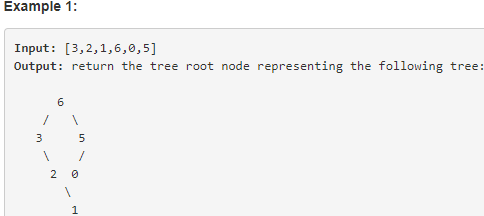
\includegraphics[width=0.6\textwidth]{example654.png}
\caption{ID 654 Given Example}
\end{figure} \\
This did not make it any clearer as to which way the subtrees should be structured. It was simple to understand that the biggest number in the subarray should be the next number in the tree and then work down in a descending order from the root node. What was hard to understand was why the two was the right child of the three, and yet zero was to the left of five, where it was to be expected. This confusion caused a delay in the solution to this question being completed. 
\subsection{Control Flow Graphs}
\label{label:CFG}
As mentioned previously, it was decided that control flow graphs would be the best way to evaluate the similarity between the code of the fundamental pattern’s, and the answer for the questions \cite{softwaretesting}. To evaluate the similarity between the pieces of code, the number of edit operations required to transform one piece of code into another was used. These edits were previously listed in section \ref{label:problemstmt}. Adding or deleting a node was counted as one operation, whilst adding or deleting any edges between nodes was also counted as one operation. The reason that control flow graphs were chosen is due to them being relatively simple to create and understand. They show the natural flow of the program and this allows for easy evaluation of similarity to a standard pattern.
\par After creating the CFG for both the standard algorithm and the solution to some answer, both CFGs were compared. The number of additions and deletions of the graph was totalled to give a number. It was decided that if this number was below ten, these two pieces of code were similar. Anything above ten was regarded as being dissimilar. In this paper an example has been included which demonstrates this between the palindrome algorithm displayed in Algorithm \ref{fig:pal} and the TwoSum algorithm displayed in Algorithm \ref{fig:twosum}. Both algorithms' CFGs have been included in Figures \ref{fig:cfgpal} and \ref{fig:cfgtwosum}. 
 \begin{figure}[h]
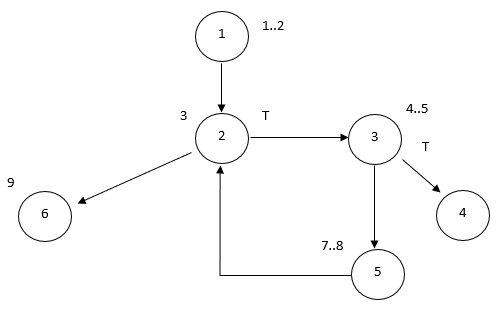
\includegraphics[width=0.6\textwidth]{CFGPalindrome.png}
\caption{Control Flow Graph for Palindrome}
\label{fig:cfgpal}
\end{figure}

 \begin{figure}[h]
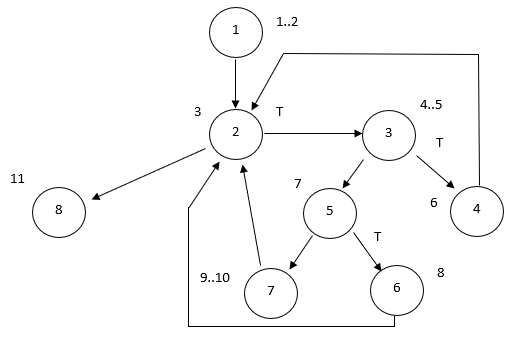
\includegraphics[width=0.6\textwidth]{CFGTwoSum.png}
\caption{Control Flow Graph for TwoSum}
\label{fig:cfgtwosum}
\end{figure}
\par Each node in the graphs represents one or more statements in the source code. The lines of code which they represent are next to each node. With regards to the two graphs, it can be seen that Figure \ref{fig:cfgpal} has a total of six nodes and six edges between the nodes. In comparison, Figure \ref{fig:cfgtwosum} has eight nodes and ten edges between them. Therefore, to transform the original pattern code into the specific version for the question there is a need for two additional nodes and four more edges. This total is therefore six edit operations. This result only proved to back up the decision that the answer to TwoSum is based off of the palindrome algorithm.
\par A second example to demonstrate the strength of CFGs is shown next. This example relates to binary search and the solution to \textbf{ID 441} Arranging Coins, which is displayed in Algorithm \ref{fig:arrangingcoins}. 
 \begin{figure}[h]
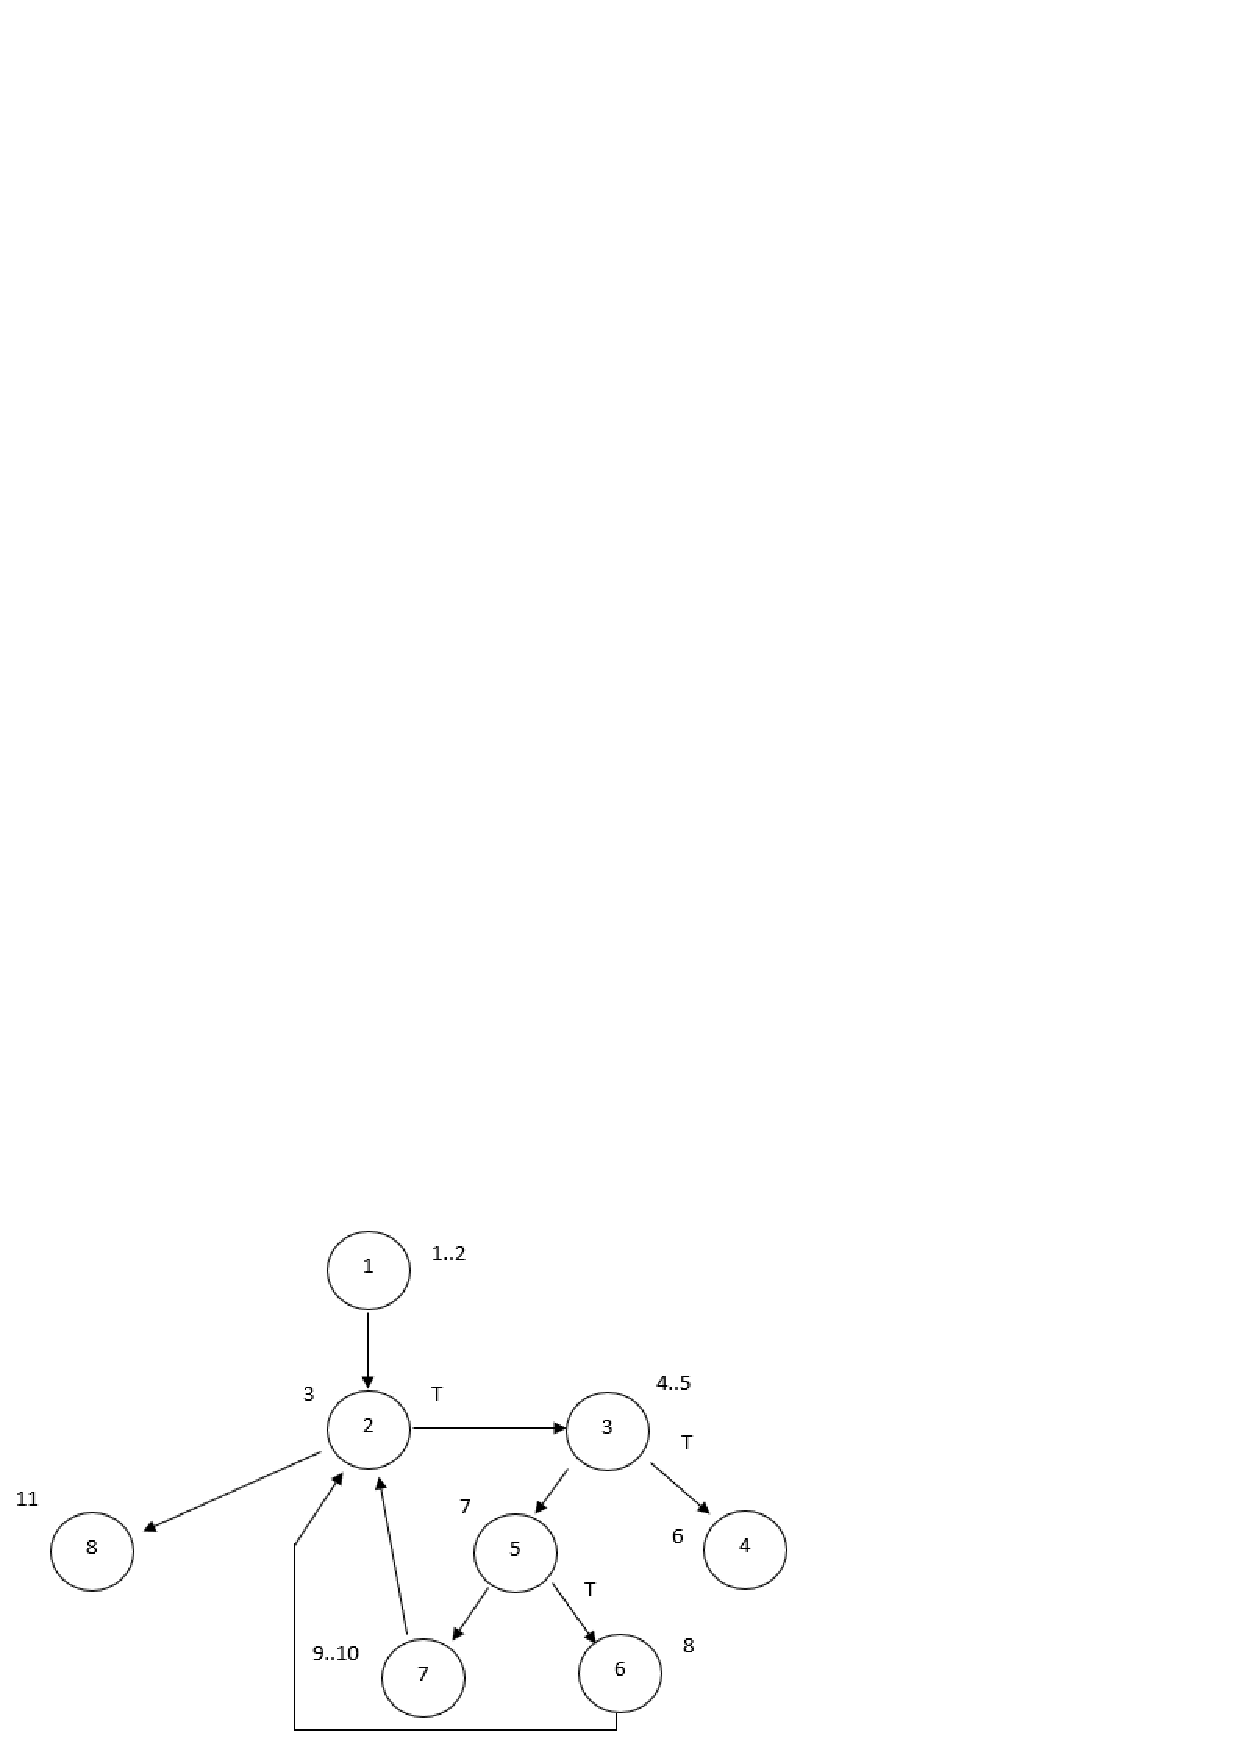
\includegraphics[width=0.6\textwidth]{CFGBinarySearch.png}
\caption{Control Flow Graph for Binary Search}
\label{fig:cfgbinarysearch}
\end{figure}
 \begin{figure}[h]
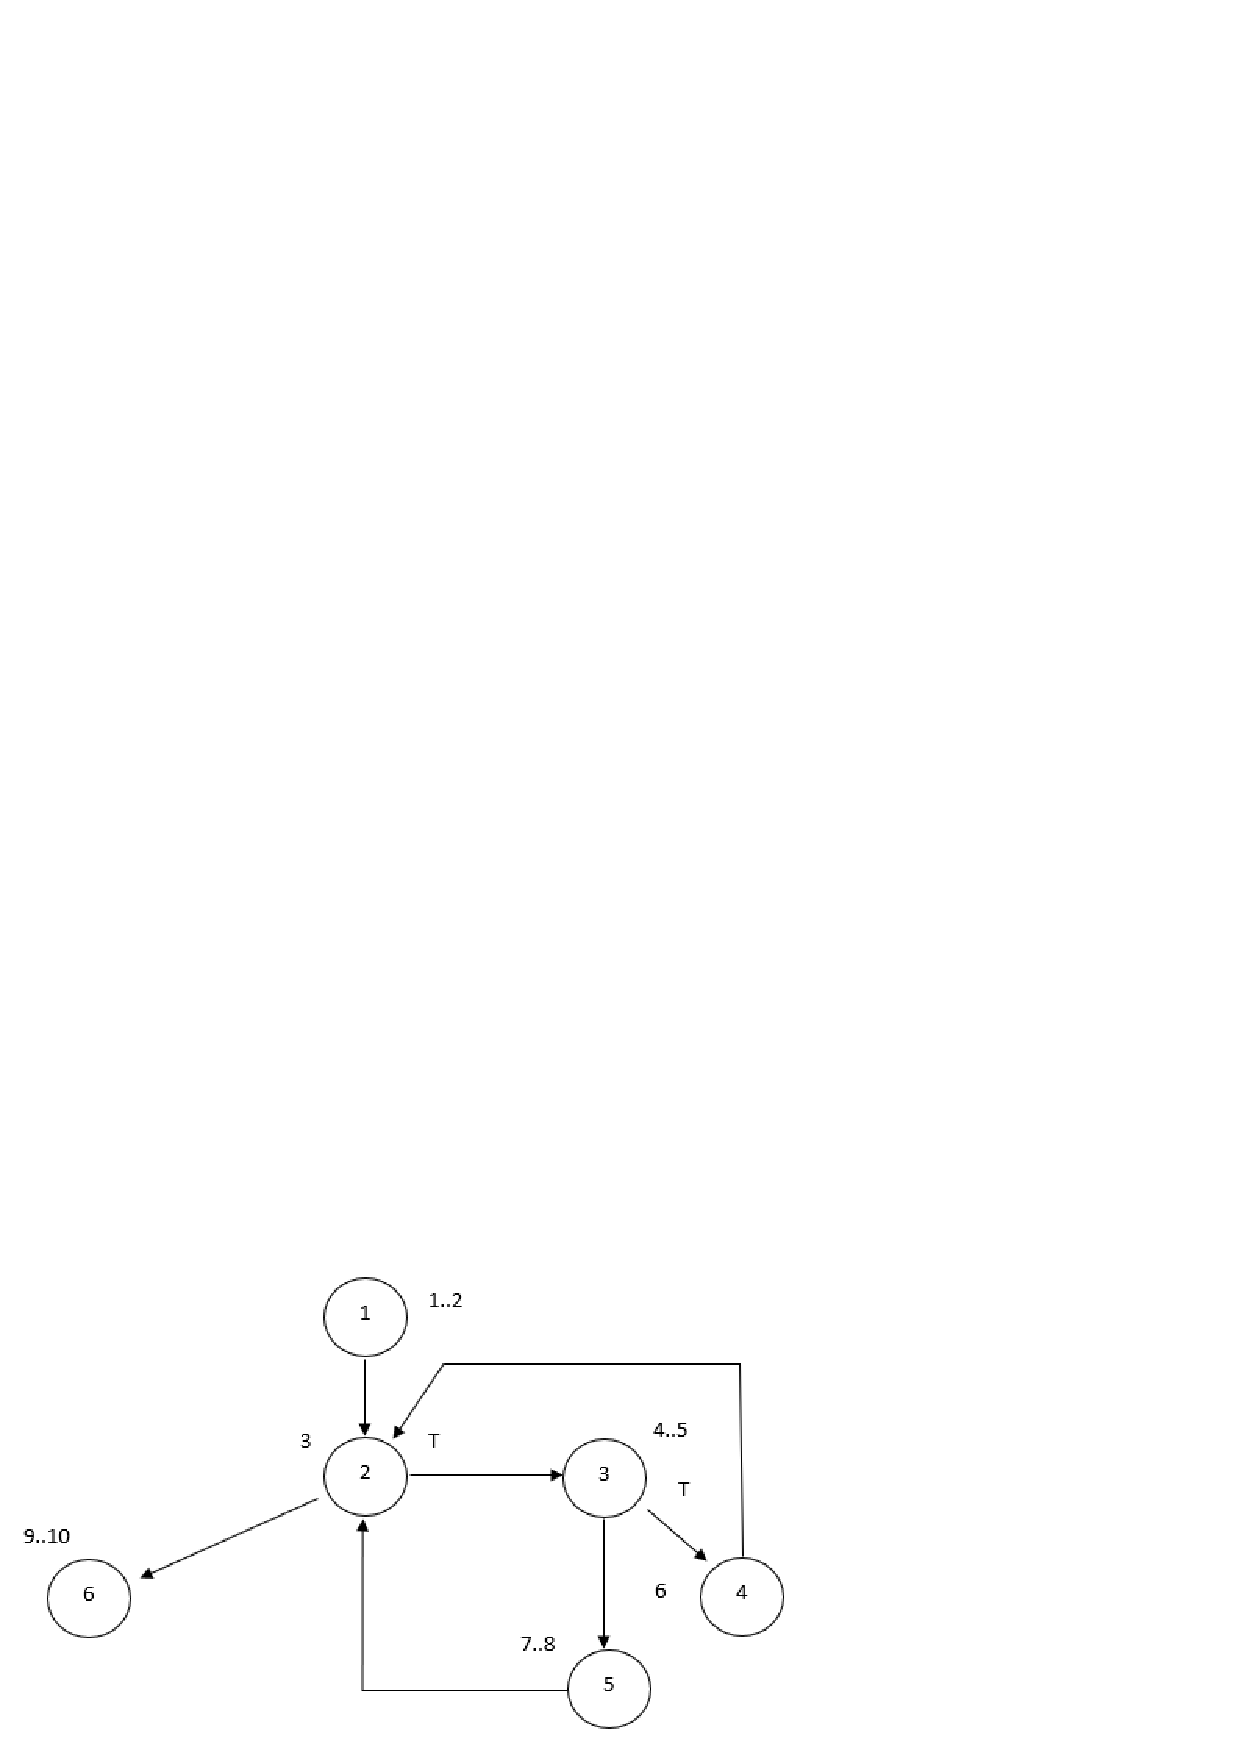
\includegraphics[width=0.6\textwidth]{CFGArrangingCoins.png}
\caption{Control Flow Graph for Arranging Coins}
\label{fig:cfgbinarysearch}
\end{figure}
\par The total number of nodes in the original pattern is eight and it contains nine edges. In the specific version for Arranging Coins there are a total of six nodes and seven edges. The total is therefore four edit operations required to transform between the two pieces of source code. 
\par The control flow graphs for each solution is provided in the appendix of this paper. Each of these graphs starts at the method signature of each method which solves the question. Therefore, the line number associated with the first node starts at line one, regardless of the line in the source code. The inline comments are also discounted when generating the graphs.
\section{Related Work}
As was mentioned earlier in this paper, there are some pieces of literature which focus on analogous topics. These include books which aim to give solutions to common programming questions \cite{mcdowell2015cracking} and the fundamentals of java \cite{markham2014java}\cite{aziz2012elements}. There are also some websites which have some mock interview questions and stage the mock interview to be similar to the normal interview process by having limited time and selected questions.

\section{Conclusion and Future Works}
In this paper we have created a guide for beginners in programming, fresh graduates and readers who wish to refresh their knowledge. This paper enables them to learn and understand some of the fundamental algorithms of programming quickly. Through learning these patterns, the reader should be able to identify solutions to a wide array of coding problems. 
\par The results of this paper have a potentially generalisable impact, yet they also have a specific impact on the key area of algorithms. The generalisable case is that this paper can apply to multiple different programming languages. Java was used to solve all the questions in this paper, but any language would have been applicable for the questions. Therefore, this paper has the potential to be useful for different programming languages. The specific case comes from this paper focusing on the algorithms and approaches to solving the problems. By showing how the algorithms, which are learned by every programmer, can be applied to multiple problems by simply changing some area of these important patterns, readers learn that specific problems can be solved using the fundamental algorithms. This will give the reader a good starting point when they are attempting to solve a question.
\par The approach taken in this paper was to solve each question manually. This process had both positives and negatives to it. The positives were that the solutions were all attempted and completed by a human, meaning that this process was similar to the interview environment. This is due to both, the interview and approach taken for this paper, having the human element of thinking of multiple ways to tackle the issues. This allowed the approach to be as valid and authentic to the real scenario of the interview as possible.
The negatives of this approach were that this manual style required a lot of human effort. This resulted in questions taking longer than expected to be completed, and questions being solved in ways which might not have been the most optimal. This method is dependent on the coding ability of the human, which depending on the topic can vary. For example, the questions relating to the advanced topic Dynamic Programming took longer to learn and be able to complete.
 In this paper there was no automatic approach to solving the questions developed. This would have been helpful for validating the solutions produced by the manual methodology. This automatic process was unable to be produced because of the time constraints of this paper. 
 \par This paper does have its limitations. As mentioned previously the approach to solve the questions can be improved. The topics which were covered are only a selection of algorithms, there are many more to be studied. For example, the questions focusing on Insertion Sort were never formally addressed in this paper. The reason this paper does not cover more topic areas is because of the time constraint for the project.
 \par With regards to future works adding to this project, it would be imperative to design and build an automatic validator. This validator tool would be used to validate the code generated for a problem, and return which standard algorithm the solution is similar to. The validator could build on the idea of the control flow graphs which counts the additions and deletions required to transform one piece of code into another. 
 To better understand the questions asked in interviews, any future works should encompass more areas of algorithms. 
 \par Overall this paper delivers a report that shows the importance and usefulness of learning the fundamental algorithms.
 

\bibliography{mybib}
\bibliographystyle{ieeetr}


\clearpage
 \appendix
\section{Source Code}
\subsection{Source Code}
\label{whatever}
\par Please see full source code in the \textit{supporting} folder.  
%\input{appendixA} % filename in curly brackets
\section{Control Flow Graphs}
\subsection{Control Flow Graphs}
\par Please see the control flow graphs subfolder inside the \textit{supporting} folder. 
\label{whatever}
%\input{appendixB} % filename in curly brackets**
 
\end{document}